\documentclass[a4paper,11pt]{article}
\usepackage{a4wide}
\usepackage{amsmath}
\usepackage{amssymb}
\usepackage{url}
\usepackage{graphicx}
%\usepackage{graphics}
\usepackage[utf8]{inputenc}
\usepackage{acronym}
%\usepackage{algorithmic}
%\usepackage{algorithm}
\usepackage{tabularx}
\usepackage{listings}

\newacro{GRASP}{Greedy Randomized Adaptive Search Procedure}
\newacro{VNS}{Variable Neighborhood Search}
\newacro{VND}{Variable Neighborhood Descent}

% \lstset{language=c,showstringspaces=true,numbers=left,numbersep=5pt}

\title{ \LARGE \bf Problem Solving and Search in AI }


\author{
\bf Partik Marschik(0625039) \\
\bf Martin Schwengerer (0625209) }

\begin{document}

\maketitle

\section{Main Algorithm}
We decided to use a \ac{GRASP} with different construction heuristics and a \emph{tabu search} as local search.
Main idea was that the tabu search, which is successfully used for the TTP\cite{Gaspero07} can be improved by starting from multiple solutions. Instead of randomly
picking these start solutions, we believe that more promising schedules may lead to more optimal results. Therefore, \ac{GRASP} with its semi-random solutios seems an 
useful and appropriated approach.

The advantages of this algorithm is that several start solutions increase the chance to start within the \emph{basin o attraction} of a good (or the optimal) solution.
In addition, a \ac{GRASP}-based search can easily be extended for multi-threading as the local searches are independent from each other.

\subsection{Problem Representation}
Solutions will be represented by a matrix $TTP$.
Rows $i$ in $TTP$ represent the round of a game.
Columns $j$ in $TTP$ represent the first team.
The value $g_{i,j}$ of a cell represents the second team.
If $g_{i,j} > 0$ then the team plays a home-game, else the team plays a out-game.
Since our indices for the matrix start at $0$ but we cannot represent $-0$ we will
store the values for $g_{i,j}$ by using the transformation
$(|g_{i,j}| + 1) \cdot \text{sgn}(g_{i,j})$.

\subsection{Construction Phase}
For the construction of our initial solution, we implemented two basic construction heuristics.
The first one (called $CA_1$) is based on the work of  \cite{Anagnostopoulos06} and constructs random schedules. These schedules fullfill the hard constraints, but ignore any additional 
requirements like the soft constraints or traveling distance between the locations.

The second approach, $CA_2$ is a \ac{GRASP} algorithm. Main idea of grasp is to extend a greedy construction heuristic with random elements such that multiple candidates for a subsequent local search are created.
For our solution, we used a multi-phase approach similar to ~\cite{Ribeiro04heuristicsfor} where in a first step, traveling patterns with virtual 
teams are created and in a subsequent step, the real teams are assigned to the virtual teams.
This assignment is based on the distance between the locations and the frequence of subsequent games in the virtual locations. 
This greedy approach is extended in a way that not always the closest locations are mapped to the most-frequent sequences, moreover a set of team-pairs (a candidate list) of the unassigned teams 
is used to select randomly te next real team-pairs for the mapping.

For creating this virtual schedule, we tested two algorithms; one based on the work of \cite{Gaspero07} which constructs a schedule with a polyon and a second one
with a randomized algorithm, as \cite{Anagnostopoulos06} suggested. For simplicity, the former will be called $VSA_1$ and the latter $VSA_2$ for the rest of the paper.
In addition, we also combinated these two methods to a new one ($VSA_{2.5}$), where the first schedules are created with $VSA_2$ and, if no further new schedules can be created
(because of the tabu list and the restricted candidate list, see below), new virtual schedules are created with $VSA_1$ which are then used again for creating ``real'' schedules with \ac{GRASP}.

One feature of the GRASP construction-algorithm is that it may create identical start solutions several times. 
This is interesting because as we use a deterministic local search, starting multiple times with the same start solution would always result in the same schedules.
To avoid this recomputation, we added a tabu list for the constrution algorithm such that if the construction phase would result in a visited start solution, this solution is dropped and a new one is created.

In addition to these two methods, our program offers a third construction algorithm ($CA_3$) which is a special case of the \ac{GRASP}-approach. As already mentioned, \ac{GRASP} determines a start solution
 by using greedy and random elements to map real teams to a virtual schedule. Our program also allows the configuration of the parameter (called \emph{alpha}) 
which ``controls'' the ratio between ``greedy'' and ``random'' elements. By setting this value to zero, the construction algorithm acts like in a greedy way and in combination with the second 
method for creating a virtual schedule ($VSA_2$), a construction method which randomly generates virtual schedules an assigns real teams in a greedy way is created.
Or course, this can also be used with $VSA_1$, but because of the lack of random elements in this algorithm, the number of different schedules creates is usually very low (except the special case that the 
distance between the team location is equal for several teams)

\subsection{Local Search}
In our program, we implement a tabu search as local search with an union of multiple neigborhoods (see below) as search space.
For the tabu list, we decided to save the complete schedules in a \emph{recency-based} manner. The reason for saving complete schedules is that some neigborhood 
(e.g. Partial Swap Rounds) may result in equal solutions as other neighborhoods, so forbidding some moves is complicated as foreign-neighborhoods must also be considered.
As a result of this decision, we do not need an aspiration criteria, as all tabu solutions have already been visited by the search and therefore, can be ignored.

\subsection{Neighborhood}
For our heuristic, we implemented and tested different neighborhoods. Some of these are based on neighborhoods used in other heuristics (like \cite{Gaspero07,rvk2008, Anagnostopoulos06}).
%For our final solution, it may be that not all of these neighborhoods are used. Moreover, we would like to evaluate the usability of these different neighborhoods with respect to size, computational effort, feasibility (does it contain only valid solutions for our hard- and soft constraints), the existence of a (simple) delta function, etc.

In detail, we use the following neighborhoods:
\subsubsection{Swapping Home/Visitor}
This simple neighborhoods ($N_1$) swaps the home/away games of two teams. This may infect the soft constraints, but never vioates any hard constraint.

\subsubsection{Swapping Teams}
This neighborhood ($N_2$) is swapping all games of two teams including the home/away status of the game. This neighborhod does not change any hard or soft constraints and 
can be seen as a 2-Opt exchange neighborhood as often used for other search problems. The size of the neighborhood is $\sum_{i=1}^{N_t-1}i$ where $N_t$ is the number of teams.

\subsubsection{Swapping Rounds}
The ``Swapping Rounds'' neighborhood ($N_3$)  exchanges all game between two rounds. This may infect the soft constraints, but never vioates any hard constraint and the 
size of this neighborhood is $\sum_{i=1}^{N_r-1}i$ where $N_r$ is the number of rounds of the schedule.

\subsubsection{Shifting Rounds}
A logical consequence of the ``Swapping Rounds'' neighborhood is to consider also a shifting of single rounds of an existing schedule ($N_4$) . 
This also may infect the soft constraints, but never vioates any hard constraint, but the number of neighbor solutions is again $\sum_{i=1}^{N_r-1}i$.

\subsubsection{Partial Swap Rounds}
This neighborhood ($N_5$) considers swapping the opponents of one team of two different rounds with the precondition that the opponents in the 
two rounds are not the same team. This move may result in a invalid state where the hard constraints are no longer fullfilled so we use a 
repair chain for re-entering the intended search space. Literature on which this neighborhood is based can be found at \cite{Gaspero07,HentenryckV06, Chen_anant}.

\subsubsection{Swap Matches}
Our last neighborhood ($N_6$) is swapping the games of two team  in one round whereby the home/away location of the teams stays the same.
This move may also lead outside our search space so a subsequent repair step is needed. This neighborhood is based on algorithms in \cite{Gaspero07, HentenryckV06}.

\subsection{Problem Relaxing}
In order to expand the search space, we decided to relax some problem constraints by allowing illegal solutions in combination with a penalty system.
Therefore, we divide the problem constraints into \emph{hard} and \emph{soft} constraints. The hard constraints are that each team plays twice against 
each other team, once at home and once as visitor and that the result is a round-robin tour. 
The soft constraint deals with the home-away-patterns, as each team has limitations about the number of consequent home (or away)-games.

We use a dynamic penalty (called \emph{shifting penalty}) which changes the weight according to the frequencies of feasible and infeasible configurations.
 Depending if the previous iterations result in a (not) allowed schedule, the penalty decreases (increases). 
This dynamic penalty mechanism is used in several other, very successful heuristics, like those by \cite{Anagnostopoulos06} or \cite{Gaspero07}.


\section{Algorithm Parameter}
As many metaheuristics, or solution suffers from a wide range of different parameters for the different party of the algorithm.
The main parameters are
\begin{center}
\begin{tabularx}{\linewidth}{| X | c | X | }
  \hline                       
  Name & Domain & Description \\   \hline     \hline    
  $L_{tabu}$ & $\mathbb{N}_{\geq0}.$ & Length of the tabu list \\ \hline    
  $N$ & $\bigcup N_x  | x \in \{1...6\}$ & Used neighborhoods for the local search \\ \hline   
  NoTabuIterations &  $\mathbb{N}_{ > 0}.$ & Number of non-improving iterations in the tabu search after which search stops. \\ \hline  
  NoGraspIterations &  $\mathbb{N}_{> 0}.$ & Number of iterations for \ac{GRASP} \\ \hline 
  Construction Method &  $\{CA_1, CA_2, CA_3\}$ & Constrction algorithm used.\\ \hline 
  VSA &  $\{VSA_1, VSA_2, VSA_{2.5}\}$ & Virtual-Schedule Construction - Constrction algorithm for creating the virtual schedules\\ \hline 
  $ \delta_P $ &  $\mathbb{Q}_{\leq0}$ & Factor for increasing and decreasing the adaptive penalty in case of consecutive illigal solutions\\ \hline 
  $P_{start}$ &  $\mathbb{Q}_{\leq0}$ &Penalty Start Value -  Initial value of the penalty factor. High values will guide the search faster to a valid solution.\\ \hline    
  $\alpha$ & $\mathbb{Q}_{\leq0}$ & Value controllig the size of the candidate list for the grasp constuction method. \\ \hline    
  \hline  
\end{tabularx}
\end{center}

\section{Parameter Configuration}
With such a high number of parameter, the question arrises which settings offers the best results on which problem instances. Therefore, we used manual and 
automatic tests for evaluating different parameter configurations.
Due to the high number of parameter, we focused on the follwing parameters for automatic testing for finding the most promising values of a predefied range:

\begin{center}
\begin{tabular}{| l | r |r | }
  \hline                       
  Name & Range & Stepsize \\   \hline     \hline    
  $L_{tabu}$ &  $0-80$& 10\\ \hline    
  $N$ &  $N_1 ... N_6$ & combination of neighborhoods\\ \hline   
  NoTabuIterations & $100-600$  & 100 \\ \hline  
  NoGraspIterations &  10-80 & 10  \\ \hline 
  Construction Method &  $CA_1, CA_2 $& - \\ \hline 
  VSA & $ VSA_1, VSA_2, VSA_{2.5}$  & \\ \hline 
\end{tabular}
\end{center}

We developed an automatic test program which evaluates the program for a specific problem instance 
by iteratively testing different configurations for one parameter. This procedure was done for multiple problem instances, leading to a big bulk of data.
As example, we plotted some aspects concerning the length of the tabu list (Figure~\ref{fig:tabu_len_cost} and Figure~\ref{fig:tabu_len_dur}) 
(see Appendix~\ref{sec:ptr} for more graphics):

\begin{figure}[htb]
  \begin{center}
    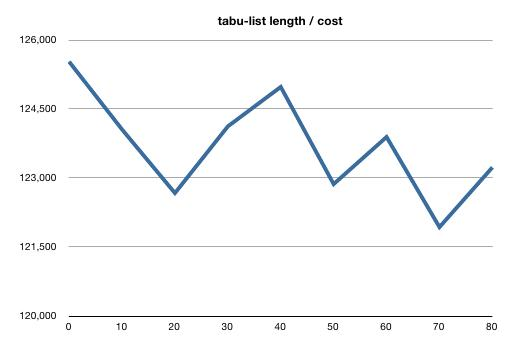
\includegraphics[width=0.8\textwidth]{images/tabulist-len-cost}
  \end{center}
  \caption{length of the tabu list vs. the resulting schedule costs}
  \label{fig:tabu_len_cost}
\end{figure}

\begin{figure}[htb]
  \begin{center}
    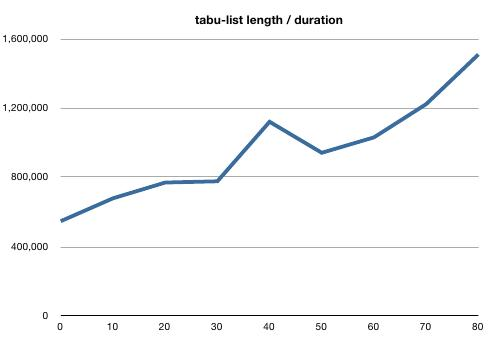
\includegraphics[width=0.8\textwidth]{images/tabulist-len-duration}
  \end{center}
  \caption{length of the tabu list vs. duration of the tabu search}
  \label{fig:tabu_len_dur}
\end{figure}

As the result of our testing, we used the followin parameter configuration for the following testing (see Table~\ref{tab:param-1}).

\begin{center}
  \begin{table}[htb]
    \begin{tabularx}{\linewidth}{| l | c | X | }
      \hline                       
      Name & Value & Note \\   \hline     \hline    
      $L_{tabu}$ & 50 & for N6.6, it is increased to 70 \\ \hline    
      $N$ &  $N_1 \cup N_2 \cup N_3 \cup N_4 \cup N_5 \cup N_6$ &  \\ \hline   
      NoTabuIterations & 500  &for N6.6, it is increased to 10000 \\ \hline  
      NoGraspIterations &  40 & less iterations may increase the number of tabu-search iterations when a very short time limit is used \\ \hline 
      Construction Method & GRASP  & for small problem instances, random construction methods also result in a global optima \\ \hline 
      VSA & $VSA_{2.5}$  & \\ \hline 
    \end{tabularx}
    \caption{Choosen parameter values after our automatic tests.}
  \label{tab:param-1}
  \end{table}
\end{center}

For other parameters, we manually choose the values as described in Table~\ref{tab:param-2}. For finding theses values, we manually testsd
our program with multiple problem instances and these values turned out to be good for most instances.
\begin{center}
 \begin{table}[htb]
  \begin{tabularx}{\linewidth}{| l | c | X | }
    \hline                       
    Name & Value & Note \\   \hline     \hline    
    $\alpha$ & $0.4$ & Depends on the problem instance \\ \hline    
    $ \delta_P $ & $ 0.125 $ & Smaller values reduce the chance to get stuck in a local optima, higher values lead the search faster to a legal solution \\ \hline    
    $P_{start}$ & $0.0$ & see $ \delta_P $ \\ \hline    
  \end{tabularx}
    \caption{Manually choosen parameter values.}
  \label{tab:param-2}
  \end{table}
\end{center}

\section{Evaluation}
As required, we tested our program on the problem instances 
\emph{NL4.4, NL6.6, NL8.8, NL10.10, NL12.12},
 each time running our program 10 times which results in the following fitnes values of the
solutions:

\begin{center}
\begin{tabular}{| l | r | r | r | r ||r | r |}
  \hline                       
  Instance& Best & Worst & Average & Median & Best Known & Derivation\\   \hline     \hline    
  NL4.4 & 8276 & 8276 & 8276 & 8276 & 8276  &  0$\%$ \\ \hline    
  NL6.6 & 23916 & 24073 & 23931,7 & 23916& 23916 &  0$\%$\\ \hline   
  NL8.8 &  40806 &41833 & 41024,2 & 40929 & 39721 & $2,7\%$\\ \hline  
  NL10.10 & 63660  &  64948 & 64311,5 & 64463 & 59436 & $6,6\%$\\ \hline 
  NL12.12 & 124097  & 127639& 125374,8 & 124725,5 & 110729 & $10,7\%$ \\ \hline
\end{tabular}
\end{center}

\section{Usage}
The program is written in Java 1.6 ans should be started via command line, e.g.
\small
\lstset{language=sh}
\begin{lstlisting}
java -jar ttp.jar data6.txt outputDir -m GRASP -c GRASP -g 40 -d 300000 -i 400
\end{lstlisting}

\section{Possible Future Work}
During out tests, we discovered that the parameter for our search strongly depend on the problem instance and on the time constraints. Therefore, 
an extention to reactive search techniques may bring large benefits on the performance of the algorithm. We especially thouht about \emph{Reactive GRASP},
 which dynamically changes the $\alpha$ value and a \emph{Reactive tabu search}. These two methods may make our solution more robust against different 
sizes and structures of different problem instances.

\small
\bibliographystyle{alpha}
\bibliography{references}

\begin{appendix}
\section{Appendix}
\subsection{Parameter Testing Results}\label{sec:ptr}

\begin{figure}[htb]
  \begin{center}
    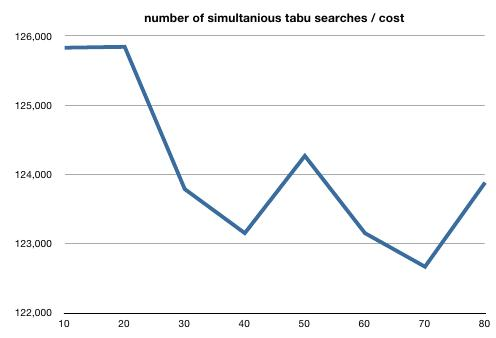
\includegraphics[width=0.8\textwidth]{images/no_grasp_iterations_costs}
  \end{center}
  \caption{no. grasp iterations and the resulting schedule costs}
  \label{fig:nograspiter}
\end{figure}

\begin{figure}[htb]
  \begin{center}
    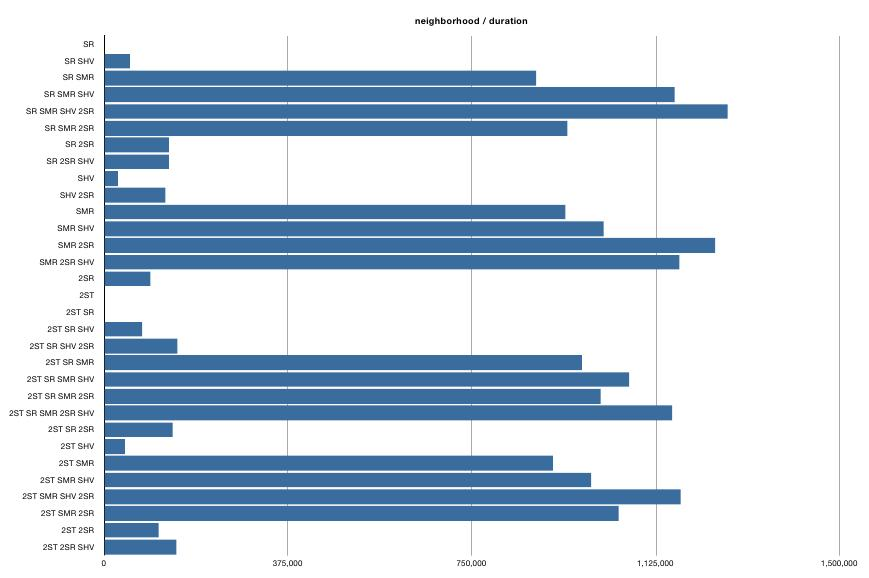
\includegraphics[width=0.8\textwidth]{images/neighborhood_duration}
  \end{center}
  \caption{no. grasp iterations and the resulting schedule costs}
  \label{fig:neighb_dur}
\end{figure}


\begin{figure}[htb]
  \begin{center}
    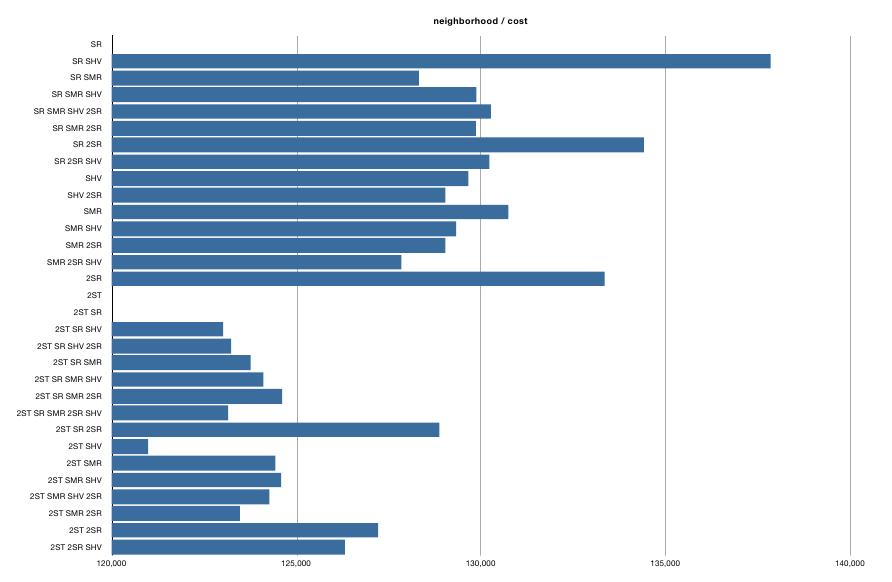
\includegraphics[width=0.8\textwidth]{images/neighborhood_cost}
  \end{center}
  \caption{no. grasp iterations and the resulting schedule costs}
  \label{fig:neighb_cost}
\end{figure}




\end{appendix}

\end{document}

